\section{Discussion}
Despite technological advances, several challenges persist in remote sensing applications for urban forestry. Occlusion remains a significant issue in dense urban environments, where buildings and infrastructure obscure portions of tree canopies from aerial sensors, on top of direct occlusion by building, building shadows can also negatively impact segmentation performance \cite{parmehrEstimationUrbanTree2016}. This limitation is particularly problematic for street trees in narrow corridors between tall buildings \cite{zhuAssessmentSpectralPolarimetric2012}. This problem is especially pronounced for smaller and younger trees.
Temporal alignment of multi-source data creates practical difficulties, as LiDAR and optical imagery are often collected at different times. This discrepancy can introduce errors when combining datasets, especially when rapid seasonal changes occur between acquisitions \cite{whiteRemoteSensingTechnologies2016}.
Accurate species identification from remote sensing data continues to challenge researchers, with classification accuracies typically ranging from $60-85\%$ depending on the number of species classes and data quality \cite{fassnachtReviewStudiesTree2016a}. This limitation affects shade modeling, as species-specific leaf characteristics, such as leaf angle and leaf color influence radiation transmission and blocking \cite{asnerSpectranomicsEmergingScience2016}.
The estimation of key parameters like Leaf Area Index (LAI) in urban contexts presents methodological challenges. Traditional optical approaches for LAI estimation developed for natural forests with a continuous canopy often perform poorly in heterogeneous urban settings with trees often separated individually or in rows \cite{yanReviewIndirectOptical2019}. LiDAR-based methods show promise but require validation against ground measurements that are laborious to collect \cite{ryuHowQuantifyTree2010}. In Amsterdam we collected a small amount of hemipsherical photography from under the tree canopy. The comparison of the hemispherical photography and the LiDAR voxelization approach reveals similar results in the calculated LAI that strengthen our LAI estimation robustness. Hemispherical photography operates on optical gap fraction analysis as shown in figure \ref{fig:hemispherical LAI}, yielding an LAI of $6.7 m²/m²$ through a gap fraction calculation, whereas LiDAR voxelization captures three-dimensional point cloud density to derive LAI through vegetation return ratios from the laser. Both capture fundamental canopy closure in different ways. Hemispherical methods excel at providing rapid validation with portable equipment and localized small-scale measurements, while LiDAR voxelization offers easier scalability and complete three-dimensional structure across large urban areas \cite{liuComparisonTerrestrialLiDAR2019} By leveraging hemispherical photography as an independent validation benchmark for both the LiDAR reference dataset and final aerial imagery predictions, we reduce systematic biases inherent to single techniques and ensure the physical validity of LAI estimates across measurement principles. The measurements from our hemispherical images, as shown in \ref{tab:Hemspherical_LAI} are in line with the range found in the Ulmus genus in our voxelization method, further underscoring the validity of our scaled voxelization method.
Data processing workflows for large urban areas demand substantial computational resources, creating implementation barriers for many municipal governments with limited technical capacity \cite{weinsteinIndividualTreeCrownDetection2019b}. The development of automated, user-friendly processing chains remains an active research area \cite{belgiuRandomForestRemote2016}.
Cost considerations also constrain the operational implementation of advanced remote sensing approaches. High-resolution LiDAR acquisition typically costs \$100-300 per km², limiting the frequency of data collection in budget-constrained municipalities \cite{holopainenTreeMappingUsing2013}.

\begin{table}[ht]
    \centering
    \begin{tabular}{ccc}
        \hline
        Tree ID & Genus & Effective LAI \\ \hline
        1 & Ulmus & 6.7 m²/m² \\
        2 & Ulmus & 4.33 m²/m² \\
        3 & Ulmus & 3.19 m²/m²\\
        4 & Ulmus & 2.92 m²/m²\\
        5 & Ulmus & 1.98 m²/m² \\ \hline
    \end{tabular}
    \caption{Example LAI measurements from 5 Ulmus trees in Amsterdam using the hemispherical photography method}
    \label{tab:Hemspherical_LAI}
\end{table}

\begin{figure}[h!]
    \centering
    % First image
    \begin{subfigure}[b]{0.41\textwidth} % Adjust width as needed for spacing
        \centering
        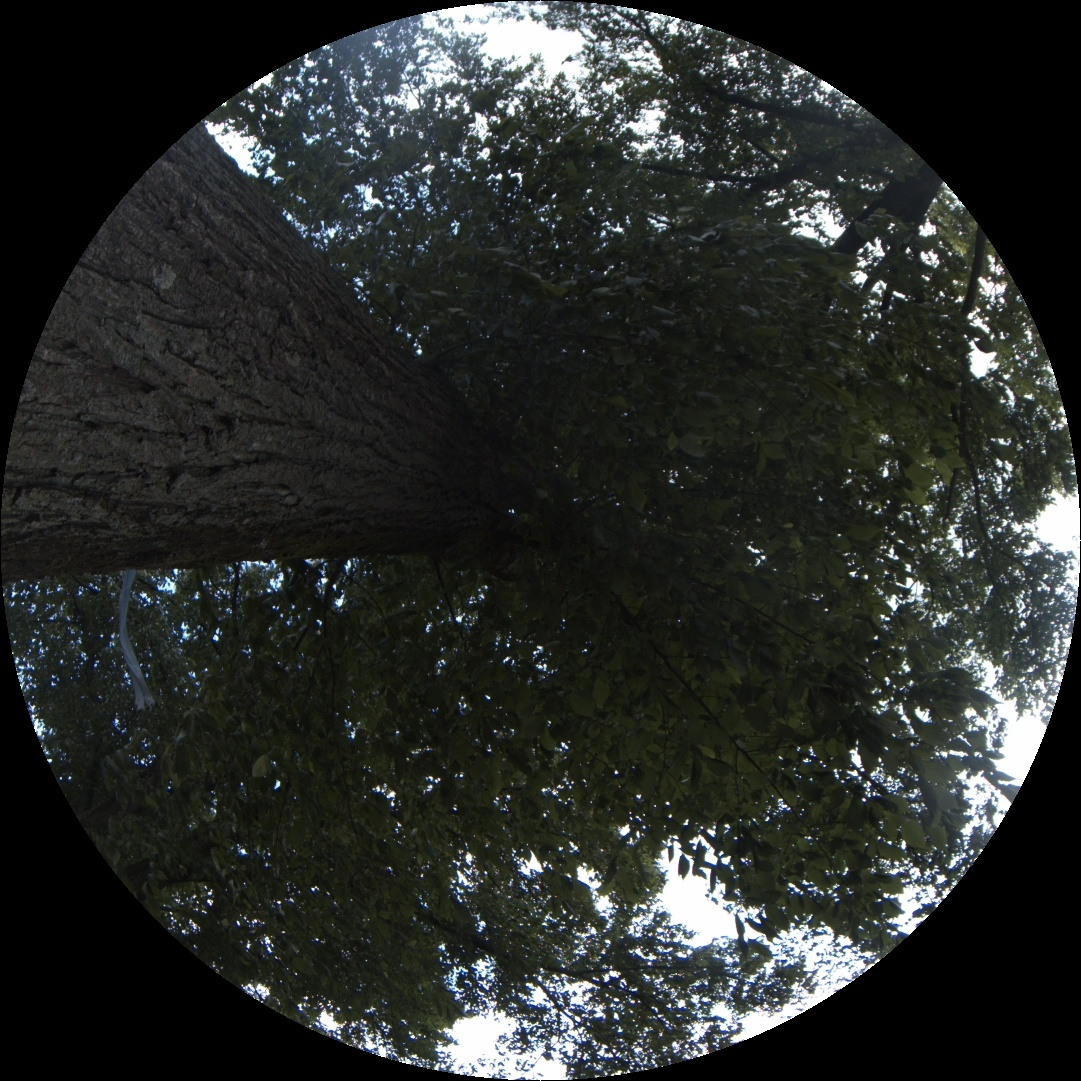
\includegraphics[width=\linewidth, height=\linewidth, keepaspectratio]{figures/methods/hemispherical_fisheye.png}
        \caption{Original Image}
        \label{fig:hemispherical_original}
    \end{subfigure}
    \hfill % Adds horizontal space between subfigures
    % Second image
    \begin{subfigure}[b]{0.48\textwidth}
        \centering
        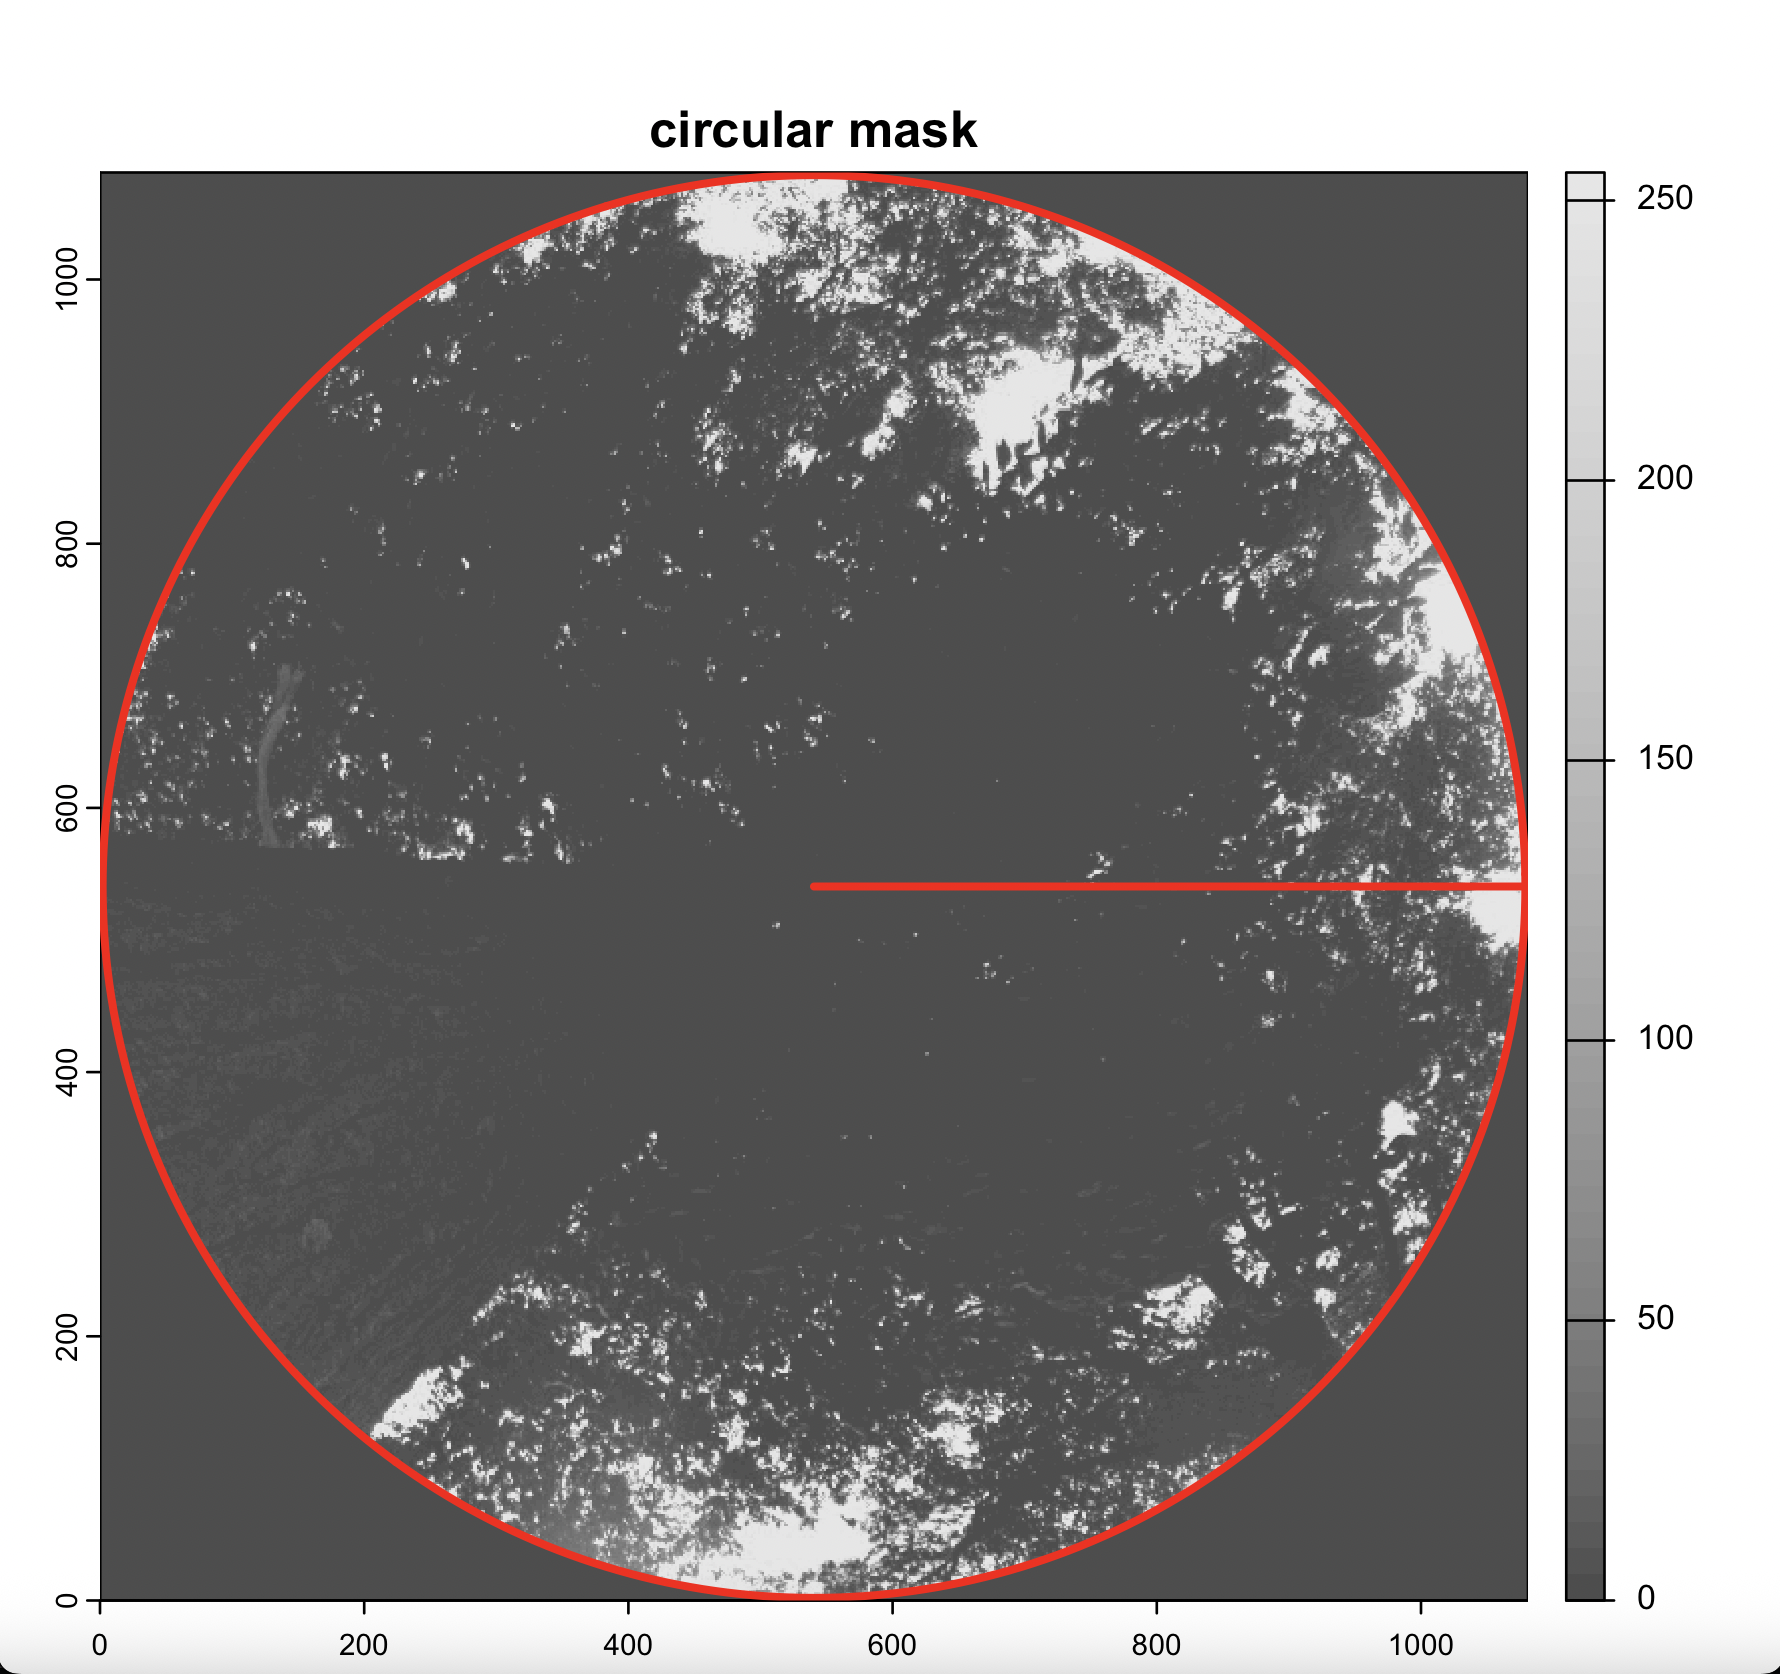
\includegraphics[width=\linewidth, height=\linewidth, keepaspectratio]{figures/methods/binarized_fisheye.png}
        \caption{Preprocessed Image}
        \label{fig:hemispherical_binarized}
    \end{subfigure}
    \caption{Two images side-by-side}
    \label{fig:hemispherical LAI}
\end{figure}
